\begin{center}
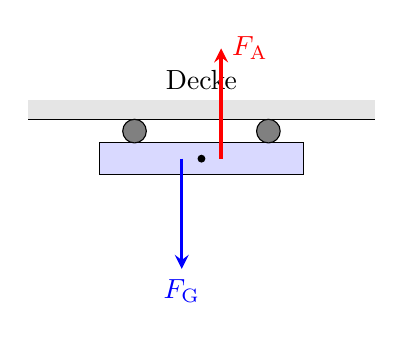
\begin{tikzpicture}[>=stealth]
 \fill[gray!20] (-2.2,2.6) rectangle (2.2,2.85);
 \draw (-2.2,2.6) -- (2.2,2.6);
 \node[anchor=south] at (0,2.85) {Decke};
 \draw[fill=blue!15] (-1.3,1.9) rectangle (1.3,2.3);
 \draw[fill=gray] (-0.85,2.45) circle (0.15) (0.85,2.45) circle (0.15);
 \fill (0,2.1) circle (0.05);
 \draw[->, very thick, blue] (-0.25,2.1) -- ++(0,-1.4) node[below] {$F_\mathrm{G}$};
 \draw[->, very thick, red] (0.25,2.1) -- ++(0,1.4) node[right] {$F_\mathrm{A}$};
\end{tikzpicture}
\hspace{1.5cm}
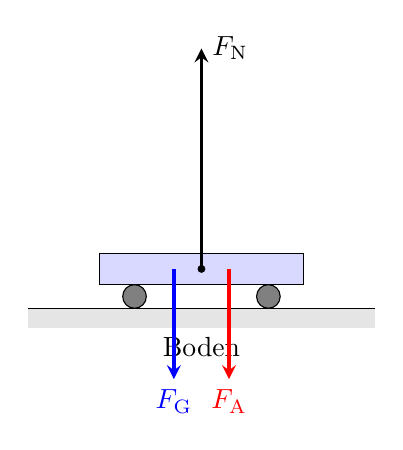
\begin{tikzpicture}[>=stealth]
 \fill[gray!20] (-2.2,0) rectangle (2.2,-0.25);
 \draw (-2.2,0) -- (2.2,0);
 \node[anchor=north] at (0,-0.25) {Boden};
 \draw[fill=blue!15] (-1.3,0.3) rectangle (1.3,0.7);
 \draw[fill=gray] (-0.85,0.15) circle (0.15) (0.85,0.15) circle (0.15);
 \fill (0,0.5) circle (0.05);
 \draw[->, very thick, blue] (-0.35,0.5) -- ++(0,-1.4) node[below] {$F_\mathrm{G}$};
 \draw[->, very thick, red] (0.35,0.5) -- ++(0,-1.4) node[below] {$F_\mathrm{A}$};
 \draw[->, very thick] (0,0.5) -- ++(0,2.8) node[right] {$F_\mathrm{N}$};
\end{tikzpicture}
\end{center}

An der Decke drückt die aerodynamische Anpresskraft $F_\mathrm{A}$ den Wagen nach oben gegen die Decke. Damit er nicht herunterfällt, muss sie mindestens so gross sein wie die Gewichtskraft:
\begin{align}
 F_\mathrm{A} &\geq \FAnF = \mFe\cdot\gE = \FAn
\end{align}
Bei normaler Fahrt (gleiche Geschwindigkeit) zeigt dieselbe Anpresskraft nach unten. Der Boden muss dann die Gewichtskraft und die Anpresskraft tragen, die Normalkraft ist also
\begin{align}
 F_\mathrm{N} &= m\,g + F_\mathrm{A} \geq \FNoF \\
   &= 2\cdot\mFe\cdot\gE \\
   &= \FNo \approx \result{\FNoP{3}{3}}
\end{align}
